\chapter{}
According to \cite{Silverman2015},to find an integer $c \in Z$ and search for Diophantine equation solutions.$y^{2}$ - $x^{3}$= $c$.Suppose we are looking for a solution in the rational numbers $x,y \in Q$.If $(x, y)$ is a solution with rational x and y and $y \neq 0$, it is simple to verify that the pair is correct.\\

$$(\frac{x^{4-8cx}}{4y^{2}},\frac{-x^{6}-20cx^{3}+8c^{2}}{8y^{3}})$$
is an answer to the identical equation in rational numbers.If the original solution is $x,y \neq 0$, then repeating the process will provide an unlimited number of different solutions.if an integer can be written using nonzero rational numbers as the difference between a square and a cube
\section{ Application of rational numbers on elliptic curves in cryptography.}
A non-singular projective curve of genus one with a determined base point is called an elliptic curve. Put a field k, such as the rational numbers Q, a finite field $F_{q}$, or even a function field C(t), in fancier terminology for the inspired. An elliptic curve E defined over k is defined as the functor that connects fields K containing k to an algebraic set.
This is Because we can make a linear change of variables, an elliptic curve is represented by a cubic equation of the form $y^{2} = x^{3} + Ax + B$ for some $A, B \in k$ fulfilling $4A^{3} + 27B^{2} \neq0$ if k is not of characteristic 2 or 3. Indeed, on the curve with z = 0, $O = (0 :1: 0)$ is the only projective point $P = (x:y:z)$.

\subsection{Fermat curves}
First of all, suppose the curve $a^{3}+b^{3}=c^{3}$ over a field $k=Q$, By substitution $a=32-8y$, $b=40+8y$, and $c=24x$, determine the elliptic curve $y^{2}+y=X^{3}-7$. The curve  $3a^{3}+4b^{3}=5c^{3}$ on the other side, is not an elliptic curve over $Q$ because it has no $Q$ rational solutions other than the degenerate one, namely $a=b=c=0$. However, this equation does define a genus one projective curve. For various exponents $n$, the curve $a^{n}+b^{n}=c^{n}$ over $Q$ has piqued people's interest. When $n$ is a large enough integer, Pierre de Fermat question if there were any nonzero $Q$ rational answers. When $n=2$, any Pythagorean Triple, such as $(a, b, c)=(3, 4, 5)$, will suffice as a desirable answer. We have seen that when $n=3$, elliptic curve arise, but this isn't the only exponent where this occurs. Surprisingly, every solution $(a,b,c)$ provides a point $P=(x, y, 1)$ on the elliptic curve $E$ when $n=7$. So $E:y^{2}+xy=x^{3}-x^{2}-107x+552$ by a hard and nontrival-substitution

$$x=49\frac{(a^{2}+b^{2}+c^{2}+ab+ac+bc)^{2}+abc(a+b+c)}{(a+b+c)^{4}}-12$$,
$$y=\frac{7(x+12)(a^{2}+b^{2}+c^{2})-x(a+b+c)^{2}}{(a+b+c)^{2}}$$
By focusing on Q-rational P on E, one can one can identify all Q-rational solutions to $a^{7} + b^{7} = c^{7}$.

\subsection{The Mordell Weil group}
The structure of the abelian group $E(K)$ is an interesting subject to study. For finite extensions $K$ of $Q$, Louis Mordell's famous theorem states that $E(K)$ is finitely created, that is, $E(K)tors Z r$ for some finite group $E(K)tors$ consisting of torsion elements and some non-negative integer $r$ called the rank.

$$y^{2}=x(x+d_{1})(x+d_{2})$$
Mazur's Theorem asserts that E(Q)tors (Z/2 Z) (Z/2 m Z) for some m = 1, 2, 3, or 4 for some m = 1, 2, 3, or 4. We can choose $T_{1} = (0 :0: 1)$ as a generator of order 2, leaving only $T_{2}$ as a generator of order 2 m to discover.The rank is much more difficult to determine: there is an injective group homomorphism, which is based on a Mordell notion.

\section{The Discrete Logarithm Problems}
There are a few unsolved issues in the field of discrete logarithms in cyclic groups. The issues arose after the Diffie-Hellman protocol was introduced in 1976. These unsolved issues are listed below.
\begin{enumerate}
	\item The Problem of Discrete Logarithms. Let G = ${g^{r}:0 \leq r \le n}$ denote an n-element random cyclic group created by $g > 1$. Find the integer r = log(s) from a primitive element g and a random element $s = g^{r} G$.
	\item The DH Problem in Computation Find $g^{rs}$ for n, g, and a random pair of elements $g^{r}$ and $g^{s}$ if you have $n and g$.
	\item DH's choice Problem. Determine whether $g^{t} = g^{rs}$ if you have n, g, and a random triple of components $g^{r}$, $g^{s}$, and $g^{t}$.
	\item Inappreciable Assumption. In polynomial time, a randomly generated triple ($g^{r}$, $g^{s}$, $g^{rs}$) $\in$ $GxGxG$ is indistinguishable from a randomly picked triple (x, y, z) $GxGxG$.
\end{enumerate}
Computing the discrete logarithm on a random cyclic group and other tough problems are examples of intractable problems. When $\in > 0$, the fastest algorithms run in $(n^{1/2}+\in)$ exponential time. The running time complexity is the number of group operations required to calculate a single discrete logarithm instance. Over the years, a lot of research has been done on this subject, but none of it has reduced the temporal complexity of the discrete logarithm in random cyclic groups. [book()].
\section{Attacks on Discrete logs}
It is easy to show that a number of these attacks are analogous to computing discrete logarithms over $GF_{p}$. Computing discrete logarithms or breaking the distribution scheme are not yet comparable to breaking the signature scheme. However, none of the assaults described in this section appear to have succeeded in cracking the system. There will be two types of attacks. In the first group, we show several methods for recovering the secret key x, and in the second group, we show some approaches for forging signatures without recovering x.
\subsection{Attacks Aiming to Recover x}
 \textit{ Attack 1:} Given ${m_{i} i= 1,2,...,l}$ information compiled with the corresponding signatures ${(r_{i},s_{i}): i=1,2,...,l}$ if an intruder tries to compute $l$ equation of the form $ m \equiv xr +ksmod(p-1)$.There are $l+1$ unknowns, and not all of the possible solutions to the system of equations have been found. Each value for x produces a system of linear equations with a diagonal matrix of coefficients, and hence each value for x provides a solution for the $k_{i}$.Recollecting $ x mod q $ requires an exponential number of message-signature pairs if $p -1$ has at least one large prime factor $q$.
Note:If any $k$ is used twice in signing, the system of equations can be solved once and $x$ retrieved. To ensure the security of the system, no value of $k$ should be used twice.

\textit{Attack 2:} Trying to compute equations of the form $a^{m} \equiv y^{r}r^{s}mod p$ always the sames as solving discrete logarithms over $GF(p)$, when both unknowns appear in the exponent.

\textit{ Attack 3:} Then the intruder will try to figure out and develop some linear dependencies in the unknown variables ${ k_{i},i=1,2,...,l}$.This is the same as solving discrete logarithms since if $k_{i} \equiv ck_{j} mod (p-1)$ hence $r_{i} \equiv {r}^{c}_{j} mod p$.if $c$ can be solved then solving discrete logarithms is easy.

\subsection{Attacks for Forging Signatures}
In order to satisfy a given document m, a forger could try to obtain r, s. If $r = a^{j} mod p$ is constant for some $j$ selected at random, computing $s$ is comparable to solving a discrete logarithm problem over $GF_{p}$. The equation can be used to compute $r$ if the forger fixes $s$ first.

	$ r^{s}y^{r} = A mod p$.
	
\textit{Attack 4:} Although it has not yet been proven that solving equation $ r^{s}y^{r} = A mod p$ for r is at least as difficult as computing discrete logarithms, we believe that solving $ r^{s}y^{r} = A mod p$ in polynomial time is not possible. The reader is challenged to come up with a polynomial time algorithm for addressing the problem $ r^{s}y^{r} = A mod p$. 

\textit{Attack 5:} We haven't been able to find an efficient solution for both r and s at the same time.

\textit{Attack 6:} The signature mechanism allows for the following attack: if an attacker knows one authentic signature for one message, he or she can create other real signatures and messages. The system is not broken because this strategy prevents an intruder from signing any message. This property can be avoided by giving m a specified structure or applying a one-way function to the message m before signing it.
The system is not broken because this strategy prevents an intruder from signing any message. This property can be avoided by giving m a specified structure or applying a one-way function to the message m before signing it.

Given a signature for a message (m),then
 
 $$a^{m} = y^{r}r^{s}mod p$$
 
Taking an integer A,B and C  arbitrarily such that (Ar -Cs) is relatively prime to p - 1.then set

$$r^{'} \equiv r^{A}a^{B}y^{C} mod p,$$
$$s^{'} \equiv sr^{'}/(Ar - Cs)mod(p - l)$$,
$$m^{'} \equiv r^{'}(Am + Bs)/(Ar - Cs)mod(p - 1)$$. 
since it is valid that $(r^{'},s{'})$ signs the message $(m^{'})$.

solve

$$y^{r^{\prime}}{r^{\prime}}^{s^{\prime}} \equiv y^{r^{\prime}}\left(r^{A}{\alpha^{B}y^{C}}\right)^{{sr^{\prime}}/(Ar-Cs)} $$

$$y^{r^{\prime}}{r^{\prime}}^{s^{\prime}} \equiv \left(y^{r^{\prime}{Ar-r^{\prime}{Cs+r^{\prime}Cs}}}r^{Asr^{\prime}}\alpha^{Bsr^{\prime}} \right)^{1/(Ar-Cs)} $$

$$y^{r^{\prime}}{r^{\prime}}^{s^{\prime}} \equiv \left(\left(y^{r}r^{s} \right)^{Ar^{\prime}}\alpha^{Bsr^{\prime}}\right)^{1/(Ar-Cs)} $$

$$y^{r^{\prime}}{r^{\prime}}^{s^{\prime}} \equiv \alpha^{m^{\prime}} $$

$$r^{\prime} \equiv {\alpha^{B}}{y^{C}}{\text{mod}\,\,p}, $$

$$s^{\prime} \equiv -r^{\prime}/C\,{\text{mod}}\,(p-1),$$

$$m^{\prime} \equiv -r^{\prime}B/C\,{\text{mod}}\,(p-1).$$

It can be shown that $(r^{\prime},s^{\prime})$ \text{signs} $(m^{\prime})$.

\subsection{Baby Step, Giant Step}
Shanks pioneered the first discrete logarithm approach, which requires around $ \sqrt n$ steps and $ \sqrt n$ storage to perform well for fairly large n. Shanks' algorithm, now known as the Baby Step, Giant Step algorithm, is as follows:
\begin{enumerate}
 \item Put an integer $m\geq$ $ \sqrt n$ and evaluate $mP$.
  \item create and save a list of ${i}_P$ for $0\leq i \leq m$
   \item Find the point $Q=jmP$ for $j=0,1...,m-1$ till one corresponds with a point from the save list.
    \item If ${i}_P=Q-jmp$, then $Q=kP$ with $k=(i+jm)(mod n)$.Hence $Q={i}_P + jmP=(i+jm)P=kp$.
\end{enumerate}
If we put an integer $m \sqrt[1]{n}$,then $m^{2} \sqrt[1]{n}$ this algorithm will work suppose that the solution $k$ is such that $0\leq k < m^{2}$.Taking $k=k_{0}+mk$ where $k_{0}\equiv k (mod m)$ and $k_{1}=(k-k_{0})/m$.when $i=k_{0} and j=k_{1}$ respectively then $0 \leq k_{1}<m$

We get
$$Q-jmp=Q-k_{1}mp=kP-k_{1}mP=(k-k_{1}m)P=k_{0}P $$
then the point corresponds with another point.

Assuming we only have an upper bound on $n=|G|$, we may use Hasse's theorem to apply this approach to an elliptic curve over $F q$.

Example.
Let $G = E(F_{41})$, where E is given by $y^{2}=x^{3}+2x+1$. Let $ P=(0,1)$ and $Q = (30,40)$. By Hasse's theorem,

suppose
$$| 41+1- E( F_{41} ) | \leq 2\sqrt{41} \implies 29.194 \leq E(F_{41}) \leq 54.806$$,
if $n=|G| \leq 54$. then we let $m=8$ since $m \geq \sqrt{54}$. Points $P_{i}$ for $1\leq i \leq 7$ are 
$$(0,1),(1,39),(8,23),(38,38),(23,23),(20,28),(26,9).$$
When $Q=jmp for j=0,1,2$ we evaluate to obtain 
$$(30,40),(9,25),(26,9),$$
Where we get a corresponding point to another point, since $j=2$ corresponds with 7P, we then get 
$$Q=(30,40)=7P+16P=23P$$. 

\subsection{ Pollard's $\rho$ Method}
The Baby Step, Giant Step algorithm has a significant disadvantage in that it requires a lot of storage space. Pollard's method takes roughly the same length of time as Baby Step, Giant Step, but requires significantly less storage. Assume that $G$ is a finite group with $|G| = n$ and $|G| = n$. Choose an erroneous function $f: G \implies G$. We start with $P_{0}$ and compute iterations from there. $P_{i+1} = f(P_{i})$. There will be some indices $i_{0}$ $j_{0}$ such that $P_{i0} = P_{j0}$ since $|G| = n$. Then,
$$P_{i0+1}=f(P_{i0})=f(P_{j0})=P_{j0+1}$$
For every $ \rho \geq 0$ $P_{i0+ \rho} = P_{j0+ \rho}$. As a result, ${P_{i}}_{i \in N}$ has a periodic period of $j_{0}-i_{0}$ or is a divisor of $j_{0}-i_{0}$. Because the procedure's graphic resembles a Greek letter, Pollard's method is called that. If $f$ is a randomly chosen random function, we should expect to find a match with j0 at most a constant times p. Then we should find a match with $j_{0}$ at most a constant times $ \sqrt n$.

\begin{figure}[h]
	\centering
	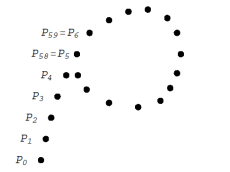
\includegraphics[scale=0.5]{pollard}
	\caption{Pollard's $\rho$ Method}
	\label{pollard}
\end{figure}
One technique implementation stores all the points $P_{i}$ until a match is found. This takes about $ \sqrt n$ of storage, which is similar to Baby Step, Giant Step. It is feasible to do significantly better with a little extra computation. The idea is that once two indices that differ by d match, all subsequent indices that differ by d will also match. Thus, for $i = 1, 2, 3,...$ we can compute pairs $(P_{i}, P_{2i})$, but we only keep the current pair. The prior pairs will not be kept.
$$P_{i+1}=f(P_{i})   and   P_{2(i+1)}=f(f(P_{2i}))$$
If $i>i_{0}$ and $i$ is a multiple of $d$, then $2_{i}$ and $i$ are a multiple of $d$ apart. As a result, $P_{i} = P_{2i}$ is a match. There is a match for $i<j_{0}$ since $d\leq j_{0}$. As a result, the number of steps required to discover a match should be at most a constant multiple of $\sqrt{n}$.
The issue is determining which function f is appropriate. Divide $G$ into $s$ distinct subsets $S_{1}, S_{2}, ...S_{s}$ of roughly equal size. $2_{s}$ randomly generated integers $a_{i}, b_{i} (mod n)$.
$$M_{i}= a_{i}P+b_{i}Q$$
define
$$f(g)=g+M_{i}$$  if $g \in S_{i}$
Choose two random integers, $a_{0}$ and $b_{0}$, and set the starting point at $P_{0} = a_{0}P + b_{0}Q$. We keep track of how these points are expressed in terms of $P$ and $Q$ when computing $P_{j}$.
If $$P_{j}=u_{j}P+v_{j}Q and P_{i+1}=P_{j}+M_{i}$$, then
$$P_{j+1}=u_{j}P+v_{j}Q+a_{i}P+b_{i}Q=(u_{j}+a_{i})P+(v_{j}+b_{i})Q$$ so
$$(u_{j+1},v_{j+1})=(u_{j}+v_{j})+(a_{i},b_{i}).$$ finding a match $P_{i0}=P_{j0}$, then
$$u_{j0}P+v_{j0}Q=u_{i0}P+v_{i0}Q \implies (u_{i0}-u_{j0})P = (v_{j0}-v_{i0})Q$$
so $gcd(v_{j0}-v_{i0},n)=d$, then
$$k \equiv (v_{j0}-v_{i0})^{-1}(u_{i0}-u_{j0})( mod n/d).$$
This results in $d$ options for $k$. Because $d$ is usually small, we can test all alternatives until $Q = kP$.
Example Let G = E(F1093) where E is the elliptic curve $y^{2} = x^{3} + x + 1$. using $s = 3$. Let $P = (0,1)$ and $Q = (413, 959)$. It can be shown that
$|P| = 1067$ and we want to find $k \in Z$ such that $Q = kP$.
Let $P_{0}=3P+5Q$, $M_{0}=4P+3Q$, $M_{1}=9P+17Q$, and $M_{2}=19P+6Q$.
Let $f: E(F_{1093}) \implies E(F_{1093})$ be defined by

$$f(x,y)=(x,y)+M_{i}$$ if $x \equiv i (mod 3)$.\\
In this case, $x$ is an integer with the value $0 \leq x \leq 1093$. It is also possible to define

$f(\infty)= \infty$. If we find $P_{0},P_{1}=f(P_{0},P_{2}=f(P_{1})$
we then get: 
$$P_{0}=(326,69),P_{1}=(727,589), P_{2}(560,365),P_{3}(1070,260)$$,
$$P_{4}=(473,903),P_{5}=(1006,951),P_{6}=(523,938), ...$$
$$P_{57}=(895,337),P_{58}=(1006,951),P_{59}=(523,938),...$$S
As a result, $P_{5}$ = $P_{58}$, and we keep track of the $P$ and $Q$ coefficients we discover.
$P_{5}=88P+46Q$  and $ P_{58}=685P+620Q$. Then
 $$P_{58}-P_{5}=567P + 574Q = \infty$$
$$Hence  |P|=1067$$
We solve 
$$-574^{-1}597 \equiv (mod 1067)$$
$$\textit{Hence, Q=499P so that k=499}$$.

\section{Elliptic Curve Domain Parameters}
There are two types of domain parameters for elliptic curves: those over $F_{p}$ and those over $F_{2m}$.Elliptic curve domain parameters over $F_{p}$ and elliptic curve domain parameters over $F_{2m}$ are detailed in \cite{brown2009standards} .Elliptic curve domain parameters can be verified as random, i.e., they are obtained in part from the output function applied to a seed value $S$. Despite the fact that taking random elliptic domain parameters are preferable, other solutions may be used for a variety of reasons, including enhanced performance.

\subsection{Elliptic Curve Domain Parameters over Fp}
The domain parameters of an elliptic curve on a finite field, say $F p$, are a sextuple:
$$T = (p, a, b, G, n, h)$$
Taking an integer $p$ and setting out the finite field $F_{p}$, two point $a,b \in F_{p}$ so setting out an elliptic curve $E(F_{p})$ is defined by:
$$E : y^{2} \equiv x^{3} + ax + b (mod p)$$
Considering a base point $G = (xG, yG)$ on $E(F_{p})$, a certain prime called n which is the order of $G$, and an integer $h$ that is
the cofactor $h = E(F_{p})/n$.
\subsection{Recommended Parameters secp192k1}
The sextuple $T = (p, a, b, G, n, h)$ provides the domain parameters of an elliptic curve over $F p$ for a Koblitz curve secp192k1, where the finite field $F p$ is specified by:
$$p = FFFFFFFF FFFFFFFF FFFFFFFF FFFFFFFF FFFFFFFE FFFFEE37$$
$$ = 2^{192}-2^{32}-2^{12}-2^{8}-2^{7}-2^{6}-2^{3}-1 $$
The curve $E$: $y^{2} = x^{3} + ax + b$ over $F_{p}$ is defined by:

$$a = 00000000 00000000 00000000 00000000 00000000 00000000$$
$$b = 00000000 00000000 00000000 00000000 00000000 00000003$$
We have the base point $G$ in a compressed form is:
$$G = 03 DB4FF10E C057E9AE 26B07D02 80B7F434 1DA5D1B1 EAE06C7D$$
the uncompressed form is:
$$G = 04 DB4FF10E C057E9AE 26B07D02 80B7F434 1DA5D1B1 EAE06C7D
9B2F2F6D 9C5628A7 844163D0 15BE8634 4082AA88 D95E2F9D$$
the order $n$ of $G$ and it cofactor are:
$$n = FFFFFFFF FFFFFFFF FFFFFFFE 26F2FC17 0F69466A 74DEFD8D$$
$$h = 01$$
$p$ is the prime, a and b are the curve's parameters, $G$ is the generator point, $n$ is the number of points in the field, and $h$ is the cofactor for all elliptic curve cryptography.

using weierstrass equation : 
$$y^{2} = x^{3} + ax + b$$
To locate an elliptic curve's private key. The diagram below illustrates how the private key can be used in conjunction with elliptic cure and algorithm knowledge..

Using Python:
\begin{figure}[h]
	\centering
	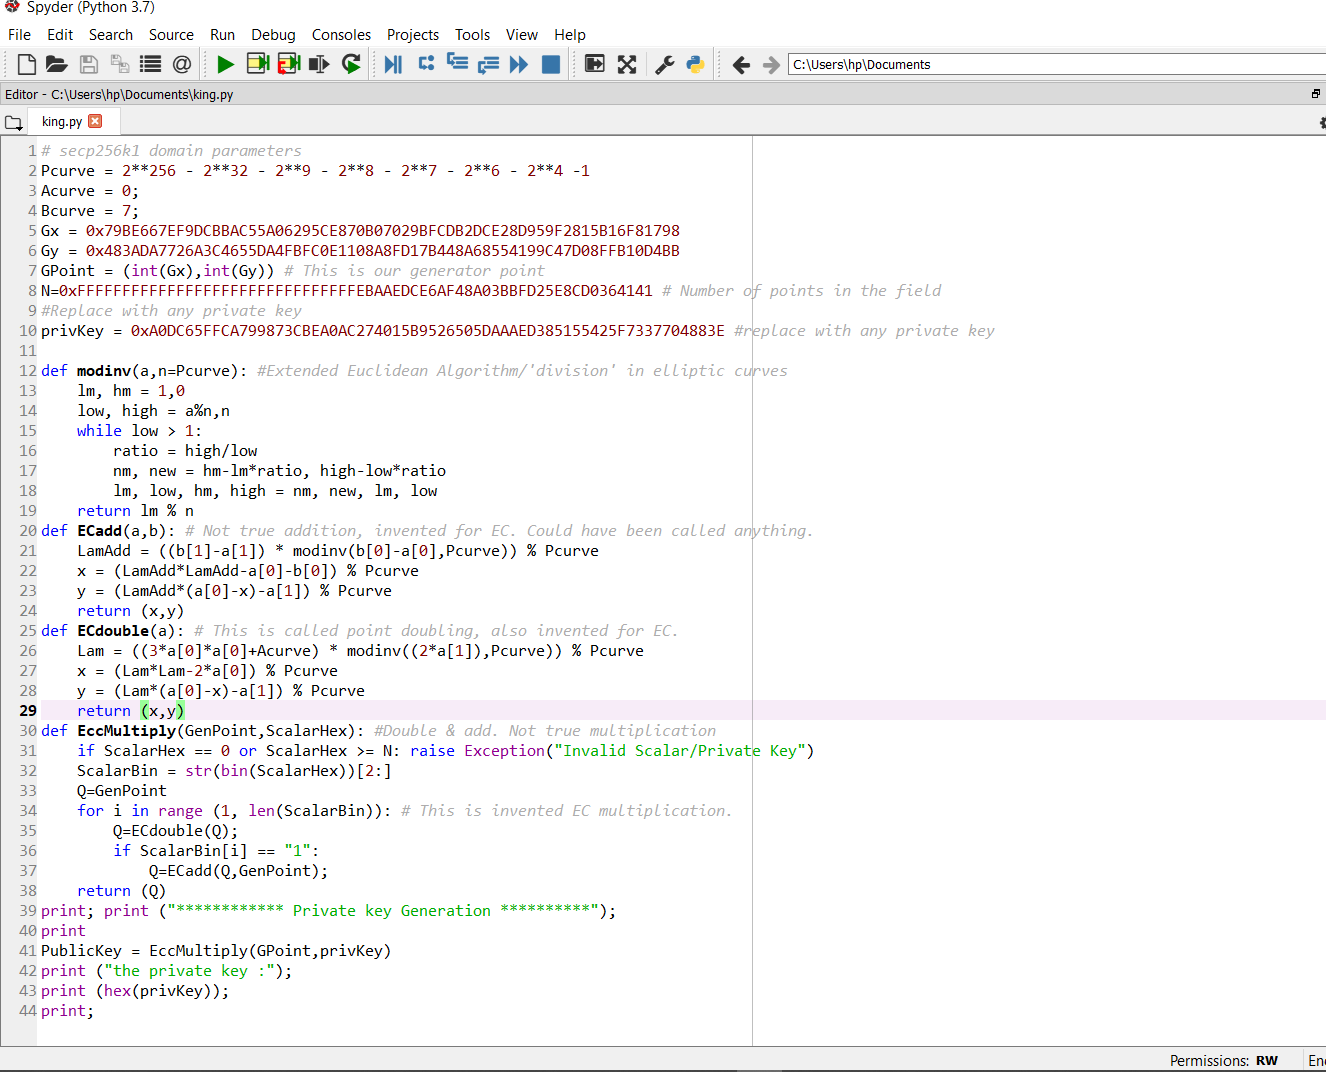
\includegraphics[width=1.5\linewidth]{private key script}
	\caption{}
	\label{fig:private key script}
\end{figure}

The result to the figure above is shown below:

\begin{figure}[h]
	\centering
	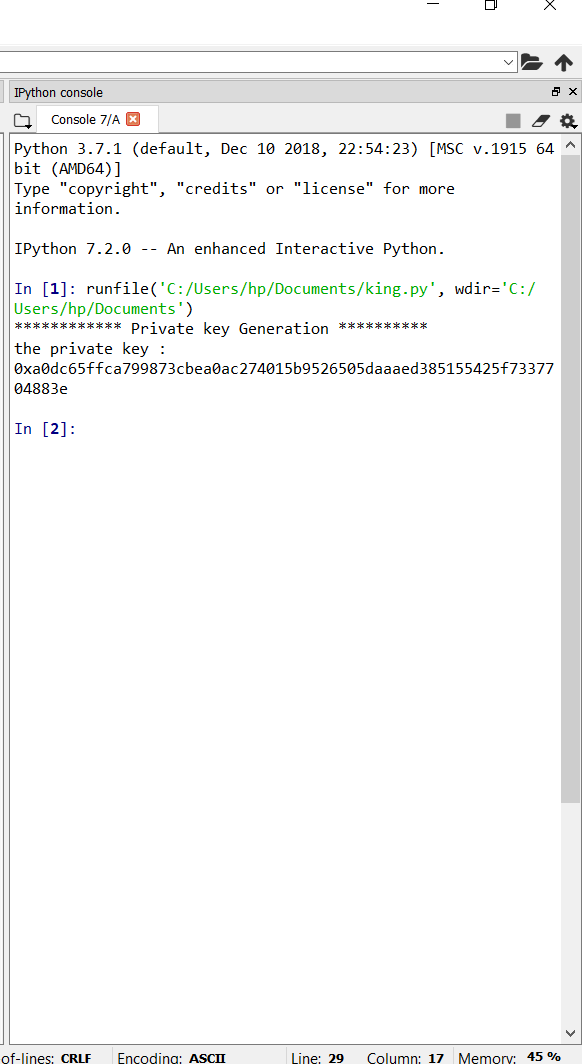
\includegraphics[width=0.9\linewidth]{private key result}
	\caption{}
	\label{fig:private key result}
\end{figure}

